
%%% Local Variables:
%%% mode: latex
%%% TeX-master: t
%%% End:

\documentclass[xcolor=svgnames,11pt]{beamer}
\usepackage[utf8]{inputenc}
\usepackage[english]{babel}
\usepackage{hyperref}
\usepackage{mathrsfs}
\usepackage{geometry}
\usepackage{listings}
\usepackage{graphicx}
\usepackage{xspace}
\usepackage{verbatim}
\usepackage{textcomp}
\usepackage{amsmath}
\usepackage{amsfonts}
\usepackage{syntax}
\usepackage{amssymb}
\usepackage{mathtools}
\usepackage{subcaption}
\usepackage{textgreek}
\usetheme{Frankfurt}
\usecolortheme{crane}

\beamertemplatenavigationsymbolsempty
\usepackage{tikz}
\usetikzlibrary{backgrounds,positioning,shapes,
  shadings,shadows,arrows,decorations.markings,calc,fit,fadings}
\input{../tikz}

\newcommand{\mysc}[1]{\textsc{#1}\xspace}
\newcommand{\coq}{\textsc{Coq}\xspace}
\newcommand{\agda}{\textsc{Agda}\xspace}
\newcommand{\ma}{\textsc{microAgda}\xspace}
\newcommand{\na}{\textsc{nanoAgda}\xspace}

\lstset{
  tabsize=4,
  aboveskip={0.5\baselineskip},
  belowcaptionskip=1\baselineskip,
  columns=fixed,
  showstringspaces=false,
  extendedchars=true,
  breaklines=true,
  frame=none,
  xleftmargin=\parindent,
  basicstyle=\scriptsize\ttfamily,
  keywordstyle=\bfseries\color{green!30!black},
  keywordstyle=[2]\bfseries\color{red!50!white},
  commentstyle=\itshape\color{purple!40!black},
  identifierstyle=\color{blue!30!black},
  stringstyle=\color{orange},
}

\lstdefinelanguage{Agda}{
  morekeywords={data,where,case},
  literate={->}{{$\to$}}1 {xx}{{$\times$}}1,
}

\lstdefinelanguage{nanoAgda}{
  morekeywords={case,of,split,rec},
  literate={->}{{$\to$}}1 {\\}{{$\lambda$}}1 {'}{`}1
    {*}{{$\times$}}1 {*0}{{$\star_0$}}2 {*1}{{$\star_1$}}2 {*2}{{$\star_2$}}2,
}
\lstset{
  aboveskip=0pt,
  belowcaptionskip=0pt,
  basicstyle=\small\ttfamily,
  escapeinside={!}{!},
}


\title{A sequent-calculus presentation of type-theory}
\author[Gabriel Radanne]{Gabriel Radanne --- Under the supervision of Jean-Philippe Bernardy}
\institute[ENS Rennes]{ENS Rennes --- Chalmers University of Technology}

\begin{document}

\begin{frame}[plain]
\titlepage
\end{frame}

\begin{frame}{Plan}
\tableofcontents%[section]
\end{frame}

\section{An Introduction to dependent types}

\begin{frame}[fragile]
  Imagine we want to define lists, but with guaranties on the length of the list.

  We have the length operation:

\alt<1>{$|$ \lstinline[language=caml,basicstyle=\ttfamily]{['a' ; 'b' ; 'c']} $| = 3$.}{$|$ \lstinline[language=caml,basicstyle=\ttfamily]{ 'a' :: 'b' :: 'c' :: []} $| = 3$.}

  \pause\pause
  \ \\We can define the head function like this in \mysc{OCaml}:
\begin{lstlisting}[language=caml]
let head x = match x with
  | [] -> failwith "PANIC" !\only<4->{\\\color{Gray}We want the type-system to ensure this doesn't happen.}!
  | (h::t) -> h
\end{lstlisting}\pause

\lstinline[language=caml,basicstyle=\ttfamily]{head l}
should only be valid if $|$\lstinline[language=caml,basicstyle=\ttfamily]{l}$|>0$.
\end{frame}

\begin{frame}[fragile]
  Let's start by natural numbers:
\begin{lstlisting}[language=Agda]
data Nat : Set where
Zero : Nat
Succ : Nat -> Nat
\end{lstlisting}\pause

\begin{lstlisting}[language=Agda]
three : Nat
three = Succ (Succ (Succ Zero))
\end{lstlisting}\pause

  We can now define a special kind of list:
\begin{lstlisting}[language=Agda]
data Vec (A : Set) : Nat -> Set where
Nil : Vec A Zero
Cons : {n : Nat} -> A -> Vec A n -> Vec A (Succ n)
\end{lstlisting}\pause

\begin{lstlisting}[language=Agda]
myVec : Vec Char three
myVec = Cons 'a' (Cons 'b' (Cons 'c' Nil))
\end{lstlisting}

\end{frame}

\begin{frame}[fragile]
\begin{lstlisting}[basicstyle=\footnotesize\ttfamily,language=Agda]
data Nat : Set where
Zero : Nat
Succ : Nat -> Nat
\end{lstlisting}
\begin{lstlisting}[basicstyle=\footnotesize\ttfamily,language=Agda]
data Vec (A : Set) : Nat -> Set where
Nil : Vec A Zero
Cons : {n : Nat} -> A -> Vec A n -> Vec A (Succ n)
\end{lstlisting}

\ \\The head function:
\begin{lstlisting}[language=Agda]
head : forall { A n } -> Vec A (Succ n) -> A
head (Cons x xs) = x
\end{lstlisting}\pause

\ \\
\begin{lstlisting}[language=Agda]
  head Nil !\color{Gray}$\gets$ This is a type error.!
\end{lstlisting}
\end{frame}

\begin{frame}[fragile]
\begin{lstlisting}[basicstyle=\footnotesize\ttfamily,language=Agda]
data Nat : Set where
Zero : Nat
Succ : Nat -> Nat
\end{lstlisting}
\begin{lstlisting}[basicstyle=\footnotesize\ttfamily,language=Agda]
data Vec (A : Set) : Nat -> Set where
Nil : Vec A Zero
Cons : {n : Nat} -> A -> Vec A n -> Vec A (Succ n)
\end{lstlisting}

\ \\When we concatenate two vectors, $|$\lstinline[language=caml,basicstyle=\ttfamily]{append l l'}$| = |$
\lstinline[language=caml,basicstyle=\ttfamily]{l}$| + |$
\lstinline[language=caml,basicstyle=\ttfamily]{l'}$|$.\pause
\begin{lstlisting}[language=Agda]
append : forall { n m A } ->
    Vec A n -> Vec A m -> Vec A (n + m)
append Nil ys = ys
append (Cons x xs) ys = Cons x (append xs ys)
\end{lstlisting}
\end{frame}

\begin{frame}{Dependent types}
What have we done?
\begin{itemize}
\item We defined a type with a {\bf term} as parameter:
\lstinline[language=Agda,basicstyle=\ttfamily]{Vec A n}.\pause
\item We used these values to enforce properties.\pause.. by type-checking.\pause
\item We manipulated these values inside the type: \lstinline[language=Agda,basicstyle=\ttfamily]{Vec A (n+m)}.
\end{itemize}\pause

Types depends on terms.
\end{frame}

\begin{frame}{Dependent types}
\begin{columns}
\column{0.6\textwidth}
Dependent types:
\begin{itemize}
\item<2-> Strongly related to Curry-Howard Isomorphism.
\item<3-> Introduce as a type-theory by Martin-Löf in 1971. Proposed as foundation of mathematics.
\item<4-> As gain popularity recently for theorem-proving with \coq,
\item<5-> but also in programming: {\only<6>{\bf}\agda}, \mysc{Idris}, \mysc{ATS},\dots
\end{itemize}
\column{0.4\textwidth}
\uncover<3->{
\begin{figure}[htbp]
  \centering
  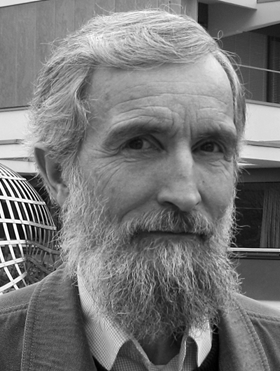
\includegraphics[width=\linewidth]{../martin-lof}

  Martin-Löf
\end{figure}
}
\end{columns}
\end{frame}

\section{Limitations of current typecheckers}
\begin{frame}
  \frametitle{Limitations of current typecheckers}
  \tableofcontents[currentsection]
\end{frame}

\subsection{Efficiency issues}
\begin{frame}{Efficiency issues}
  \agda's type checker uses a natural deduction style:
  \begin{itemize}
  \item Inference duplicates parts of terms.
  \item These parts are not shared in the \agda core representation anymore.
  \item Typechecking must be done multiple time, causing performance penalties.
  \end{itemize}
  \pause
  \begin{figure}
    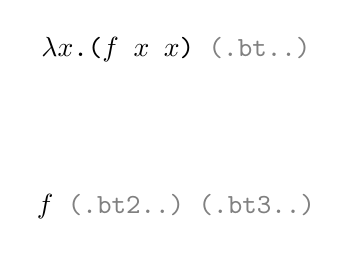
\begin{tikzpicture}
      \node[anchor=center] (lambda) at (0,0) {
        \texttt{$\lambda{}x$.($f$ $x$ $x$) {\color{Gray}(.\tikzcoord{bt}..)}}
      };
      \node<3>[anchor=center, text centered] (lambda2) at (0,-2) {
        \texttt{$f$\ {\color{Gray}(.\tikzcoord{bt2}..)\ (.\tikzcoord{bt3}..)}}
      };
    \end{tikzpicture}
    \centering
  \end{figure}
  \begin{tikzpicture}[remember picture, overlay]
    \node[xshift=0.1cm,yshift=-0.2cm, coordinate] (bt') at (bt) {} ;
    \draw<3>[remember picture, -latex] (bt') to[out=-90,in=90] ($(bt2)+(0.1,0.3)$) ;
    \draw<3>[remember picture, -latex] (bt') to[out=-90,in=90] ($(bt3)+(0.1,0.3)$) ;
  \end{tikzpicture}
\end{frame}

\subsection{The ``case decomposition'' issue}
\begin{frame}{The ``case decomposition'' issue}
  Natural deduction style makes propagating typing constraints to subterms difficult.

  For example, \agda's typechecker has no knowledge of which branch was taken while it typechecks the body of a case.
  \begin{center}
    \begin{minipage}{0.9\textwidth}
      \lstinputlisting[basicstyle=\ttfamily,language=Agda]{../poster/case.agda}
    \end{minipage}
  \end{center}
\end{frame}

\subsection{The monolithic approach}
\begin{frame}{The monolithic approach}
  \agda currently does not have a core language that can be reasoned about and formally verified.

  \coq, on the other hand, is built as successive extensions of a core language (CIC).
  \begin{figure}[htbp]
    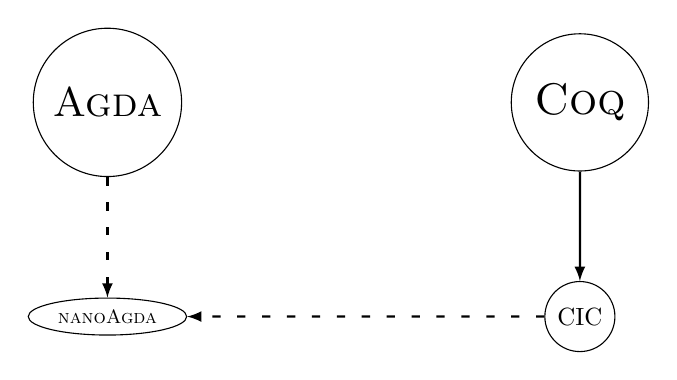
\begin{tikzpicture}[yscale=0.4, xscale=0.4]
      \node[draw, circle, scale=1.6] (Coq) at (8,3) {\coq} ;
      \node[draw, circle, scale=0.9] (CCC) at (8,-3.8) {CIC} ;
      \node[draw, circle, scale=1.5] (agda) at (-7,3) {\agda} ;
      % \node[draw, ellipse, scale=0.9] (ma) at (-7,3) {\ma} ;
      \node<2>[draw, ellipse, scale=0.7] (na) at (-7,-3.8) {\na} ;
      \draw[-latex,thick] (Coq) -- (CCC) ;
      % \draw[-latex,thick] (ma) -- (na) ;
      \draw<2>[-latex,thick, loosely dashed] (agda) to (na) ;
      \draw<2>[-latex,thick, loosely dashed] (CCC) to (na) ;
    \end{tikzpicture}
    \centering
  \end{figure}
\end{frame}

\section{\na and \ma}

\subsection{Goals}
\begin{frame}{Goals}
  Our goals are to have a language that is:
  \begin{itemize}
  \item<1-> A type-theory: Correctness should be expressible via types.
  \item<2-> Low-level: One should be able to translate high-level languages into this language while retaining properties such as run-time behaviour, complexity, etc.
  \item<3-> Minimal: The language should be well defined and it should be possible to formally verify the type-checking algorithm.
  \end{itemize}
\end{frame}

\subsection{\na}
\begin{frame}[fragile]{\na}
\begin{columns}
\column{0.5\textwidth}
\lstinputlisting[language=nanoAgda]{../poster/Lam.agda}
\centering in \agda
\column{0.7\textwidth}
\lstinputlisting[basicstyle=\scriptsize\ttfamily,language=nanoAgda]{../../examples/010-Lam.na}
\centering in \na
\end{columns}
\end{frame}

\begin{frame}{Sequent calculus}
  There are various definitions of sequent calculus. Here, we mean that every intermediate results or sub-terms are bound to a variable.
  \alt<2->{
    \begin{figure}
      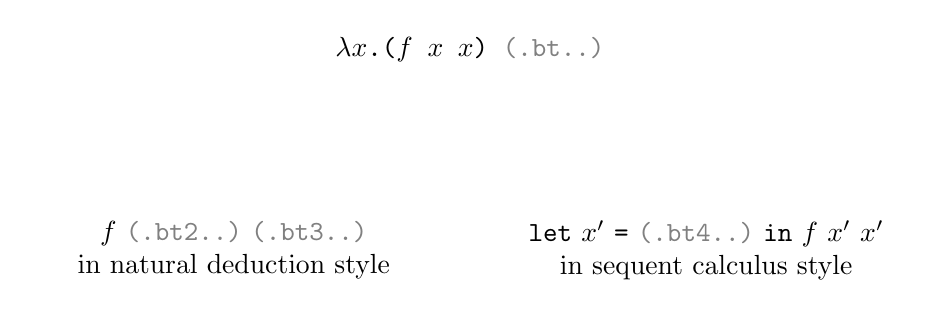
\begin{tikzpicture}[yscale=1.7]
        \node (lambda) at (0,0) {
          \texttt{$\lambda{}x$.($f$ $x$ $x$) {\color{Gray}(.\tikzcoord{bt}..)}}
        };
        \node[text centered, text width=5cm] (lambda2) at (-3,-1.5) {
          \texttt{$f$\ {\color{Gray}(.\tikzcoord{bt2}..)\ (.\tikzcoord{bt3}..)}}\\
          in natural deduction style
        };
        \uncover<3->{\node[text centered, text width=5cm] (lambda3) at (3,-1.5) {
          \texttt{let $x'$ = {\color{Gray}(.\tikzcoord{bt4}..)}\ in $f$ $x'$ $x'$}\\
          in sequent calculus style
        };}
      \end{tikzpicture}
      \centering
    \end{figure}
  \begin{tikzpicture}[remember picture, overlay]
    \node[xshift=0.1cm,yshift=-0.2cm, coordinate] (bt') at (bt) {} ;
    \draw[remember picture, -latex] (bt') to[out=-90,in=80] ($(bt2)+(0.1,0.3)$) ;
    \draw[remember picture, -latex] (bt') to[out=-90,in=60] ($(bt3)+(0.1,0.3)$) ;
    \draw<3->[remember picture, -latex] (bt') to[out=-90,in=90] ($(bt4)+(0.1,0.3)$) ;
  \end{tikzpicture}
  }{\begin{figure}[htbp]
      \lstinputlisting[language=Caml]{seq.ml}
      \centering
    \end{figure}
  }
\end{frame}

\begin{frame}[shrink]{Presentation of the language}
\begin{figure}[!h]
  \begin{subfigure}[b]{0.3\linewidth{}}
    \begin{align*}
      \ensuremath{\text{t}} ::=\:&\ensuremath{\overline{\text{x}}}\\ |\:&\ensuremath{\text{\texttt{let}}\:\text{x}=\text{d}\:\text{\texttt{in}}\:\text{t}}\\ |\:&\ensuremath{\text{\texttt{case}}\:\text{x}\:\text{\texttt{of}}\:\{\text{\ensuremath{(\text{`l}\to{}\text{t})}\ensuremath{\text{*}}}\}}\\ |\:&\ensuremath{\text{\texttt{let}}\:\overline{\text{x}}=\text{c}\:\text{\texttt{in}}\:\text{t}}
    \end{align*}
    \caption{Terms}
  \end{subfigure}
  \begin{subfigure}[b]{0.25\linewidth{}}
    \begin{align*}
      \ensuremath{\text{d}} ::=\:&\ensuremath{\text{x}} \: \ensuremath{\overline{\text{y}}}\\ |\:&\ensuremath{\text{x}\mathsf{.1}} \: | \: \ensuremath{\text{x}\mathsf{.2}} \\ |\:&\textcolor{red}{\ensuremath{\overline{\text{x}}:\overline{\text{y}}}}
    \end{align*}
    \caption{Destructions}
  \end{subfigure}
  \begin{subfigure}[b]{0.3\linewidth{}}
    \begin{align*}
      \ensuremath{\text{c}} ::=\:&\ensuremath{\text{x}}\\|\:&\ensuremath{\lambda{{}}} \ensuremath{\text{x}} . \ensuremath{\text{t}}\:|\:\ensuremath{(\text{x}:\overline{\text{y}})\to{}\text{t}}\\|\:&(\ensuremath{\overline{\text{x}}},\ensuremath{\overline{\text{y}}})\:|\:\ensuremath{(\text{x}:\overline{\text{y}})\times{}\text{t}}\\|\:&\ensuremath{\text{`l}}\:|\:\ensuremath{\{\text{`l}\}}\\|\:&\ensuremath{\star{}} \ensuremath{_{\text{i}}}
    \end{align*}\caption{Constructions}
  \end{subfigure}
\end{figure}
\end{frame}


\begin{frame}[fragile]{How to encode sumtypes}
\begin{columns}
\column{0.5\textwidth}
\begin{lstlisting}[language=Agda]
data MySumtype (s : Set) : Set where
  Foo : s -> MySumtype s
  Bar : MySumtype s
\end{lstlisting}
\centering in \agda
\column{0.5\textwidth}
TODO
\end{columns}
\end{frame}

%TODO Act interactive highlighting
\subsection{\ma}
\begin{frame}[fragile]{\ma}
A new syntax, easier to manipulate, and that can be translated easily into \na.

\begin{columns}
\column{0.5\textwidth}
\lstinputlisting[language=nanoAgda]{../../examples/010-Lam.ma}
\centering in \ma
\column{0.7\textwidth}
\lstinputlisting[basicstyle=\scriptsize\ttfamily,language=nanoAgda]{../../examples/010-Lam.na}
\centering in \na
\end{columns}

\end{frame}


\begin{frame}[fragile]{How to encode sumtypes -- $2^{nd}$ edition}
\begin{columns}
\column{0.5\textwidth}
\begin{lstlisting}[language=Agda]
data MySumtype (s : Set) : Set where
  Foo : s -> MySumtype s
  Bar : MySumtype s
\end{lstlisting}
\centering in \agda
\column{0.56\textwidth}
\lstinputlisting[basicstyle=\scriptsize\ttfamily,language=nanoAgda]
{../../examples/datatype.ma}
\centering in \ma
\end{columns}
\end{frame}

\begin{frame}[fragile]{How to encode stupidly simple sumtypes}
\begin{columns}
\column{0.56\textwidth}
\begin{lstlisting}[language=Agda]
data SimpleSum : Set where
  Foo : Nat -> SimpleSum
  Bar : Nat -> SimpleSum
\end{lstlisting}
\centering in \agda
\column{0.56\textwidth}
\begin{lstlisting}[language=nanoAgda]
TERM
  { 'Foo ; 'Bar } * Nat
Type
  *0
\end{lstlisting}
\centering in \ma
\end{columns}
\end{frame}

%TODO Act interactive highlighting
\begin{frame}[fragile]{How to encode sumtypes -- $2^{nd}$ edition}
\begin{columns}
\column{0.5\textwidth}
\begin{lstlisting}[language=Agda]
data MySumtype (s : Set) : Set where
  Foo : s -> MySumtype s
  Bar : MySumtype s
\end{lstlisting}
\centering in \agda
\column{0.56\textwidth}
\lstinputlisting[basicstyle=\scriptsize\ttfamily,language=nanoAgda]
{../../examples/datatype.ma}
\centering in \ma
\end{columns}
\end{frame}

\subsection{Results}
\begin{frame}{Results}
\begin{itemize}
\item We implemented a typechecker and evaluator for \na.
\item We introduced a new intermediate language: \ma.
\item We exhibited some examples that don't typecheck in \agda but typecheck in \na.
\end{itemize}
\end{frame}

\section{Conclusion}
\begin{frame}{Future work}
\begin{itemize}
\item Precisely evaluate the efficiency of this new approach.
\item Prove subject-reduction of \na (in \coq).
\item Introduce recursion.
\item Experiment with extensions of the type system (linear, colors,\dots).
\end{itemize}
\end{frame}

\begin{frame}[plain]
  \begin{center}
    \Huge Questions ?
  \end{center}
\end{frame}


\end{document}
